\section{The List of Concepts}
\begin{enumerate}
  \item \textbf{Calculator} \\ The main concepts that centralize all other concepts.
  \item \textbf{IrrationalNumber} $<<Abstract>>$ \\ Holds value of an irrational number.
  \item \textbf{SilverRatioNumber} \\ Holds value of Silver Ratio Number. \\ And it is a extended from the base concept $IrrationalNumber$.
  \item \textbf{Pi} \\ Holds value of Pi Number. \\ And it is a extended from the base concept $IrrationalNumber$.
  \item \textbf{EulerNumber}  \\ Holds value of Euler's Number. \\ And it is a extended from the base concept $IrrationalNumber$.
  \item \textbf{Operator} $<<Abstract>>$ \\ Represents the operators.
  \item \textbf{Adder}  \\ Represents addition operator. \\ And it is a extended from the base concept $Operator$.
  \item \textbf{Subtractor} \\ Represents subtraction operator. \\ And it is a extended from the base concept $Operator$.
  \item \textbf{Multiplier} \\ Represents multiplication operator. \\ And it is a extended from the base concept $Operator$.
  \item \textbf{Divider} \\ Represents division operator. \\ And it is a extended from the base concept $Operator$.
  \item \textbf{Operand} \\ Represents the operands.
  \item \textbf{Expression} $<<Abstract>>$ \\ Represents expressions and evaluate expression function.
  \item \textbf{AreaOfRegularOctagonExpression} \\ Represents expression to calculate area of regular octagon using $SilverRatioNumber$. \\ And it is a extended from the base concept $Expression$.
  \item \textbf{IrrationalValueGenerationExpression} \\ Represents expression to calculate the value of irrational number up to given certain decimal places. \\ And it is a extended from the base concept $Expression$.
  \item \textbf{IrrationalAlgebraicExpression} \\ Represents irrational algebraic expressions. \\ And it is a extended from the base concept $Expression$.
  \item \textbf{IrrationalArithmaticExpression} \\ Represents irrational arithmetic expressions. \\ And it is a extended from the base concept $Expression$.
  \item \textbf{AreaOfCircleExpression} \\ Represents expression to calculate area of a circle using $Pi$. \\ And it is a extended from the base concept $Expression$.
\end{enumerate} 

\section{Relationships between the Concepts}
\begin{enumerate}
\item IrrationalNumber, Operator and Operand \textbf{are part of} Calculator \textbf{(Aggregation Relationship)}.
\\ Calculator \textbf{has one or more} IrrationalNumber, Operator and Operand.
\item SilverRatioNumber, EulerNumber and Pi \textbf{extends} \textbf{(Generalization Relationship)}.
\item Adder, Subtractor, Multiplier and Divider \textbf{extends} Operator \textbf{(Generalization Relationship)}.
\item Expression \textbf{uses one or more} Operand and Operator \textbf{(Association Relationship)}.
\item AreaOfRegularOctagonExpression, IrrationalValueGenerationExpression, IrrationalAlgebraicExpression, IrrationalArithmaticExpression and AreaOfCircleExpression \textbf{extends} Expression \textbf{(Generalization Relationship)}.
\item AreaOfRegularOctagonExpression \textbf{uses one} SilverRatioNumber \textbf{(Association Relationship)}.
\item AreaOfCircleExpression \textbf{uses one} Pi \textbf{(Association Relationship)}.
\end{enumerate} 
\section{A Domain Model diagram}
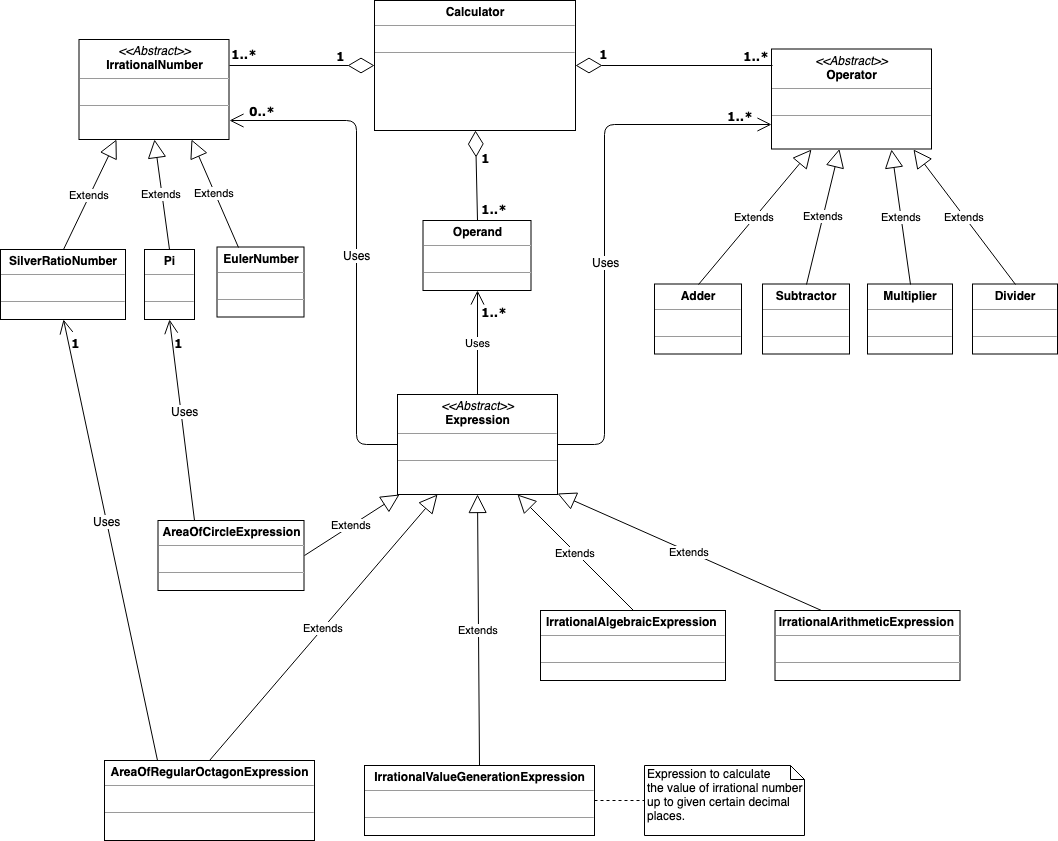
\includegraphics[width=1.0\textwidth]{images/domainmodel.png}